%%% AUTHOR: ATAKAN

\subsection{Interface Viewpoint}
\paragraph{}
\normalsize

	Interface viewpoint can be decomposed into three major components. First, the data importer module is responsible for importing voxel position values, voxel intensity values and edges (archlengths). The file format will be MATLAB file format; however, this module can be extended with ability to handle other file formats, namely CSV, raw text, eg. Second, the filtering module is responsible for preparing data to be shown on the screen smoothly. This includes down-sampling, quantization, edge boundling e.g. techniques. The output of this component will be ready-to-draw voxel position parameters, voxel intensity values and edges (archlengths). Lastly, visualization component will use 3D rendering engine and draw the image to the screen. This is visualized using UML component diagram below.\\
    
    \begin{tikzpicture} 
	\begin{umlcomponent}[x=0,y=0]{Data Importer Module} 

	\end{umlcomponent} 

	\begin{umlcomponent}[x=10,y=0]{Filtering Module} 

	\end{umlcomponent} 

	\begin{umlcomponent}[x=5,y=-7]{Visualizing Module} 

	\end{umlcomponent} 

	\umlassemblyconnector[interface=DataPacket]{Filtering Module}{Data Importer Module}

	\umlVHVassemblyconnector[interface=DataPacket]{Visualizing Module}{Filtering Module}
    
	\end{tikzpicture}


Expected user interface is depicted at Figures \ref{fig:mainWindow}, \ref{fig:fileMenu}, \ref{fig:editMenu}, \ref{fig:viewMenu} and \ref{fig:helpMenu}. There will only be one main screen. Left pane is the image plane and user will be able to interact with this plane by the hand cursor to rotate the 3D image. On the right pane, controls for rotating and zooming will be placed. Layer depth, transparency and voxel size will be customizable through a slider. Filter group lists the filters available (namely down-sampling, quantization, edge boundling e.g.). Note that as the research continues new filter will be added. Filter options can be set up through edit menu -> Filters. Region can be selected using a dropdown menu. Available options will be whole brain, frontal lobe, parietal lobe, occipital lobe, temporal lobe and limbic lobe. Note that however, these region options are tentative. Lastly, a suitible view for colorblind people will be generated if the related option is enabled. \\

Our intention for the behaviour of these right pane options is as follows. As any option change occurs, the related action will be triggered instantaneously. However, as the processing might take some time, an popup box indicating work done will be shown.


\begin{figure}[h!]
\centering
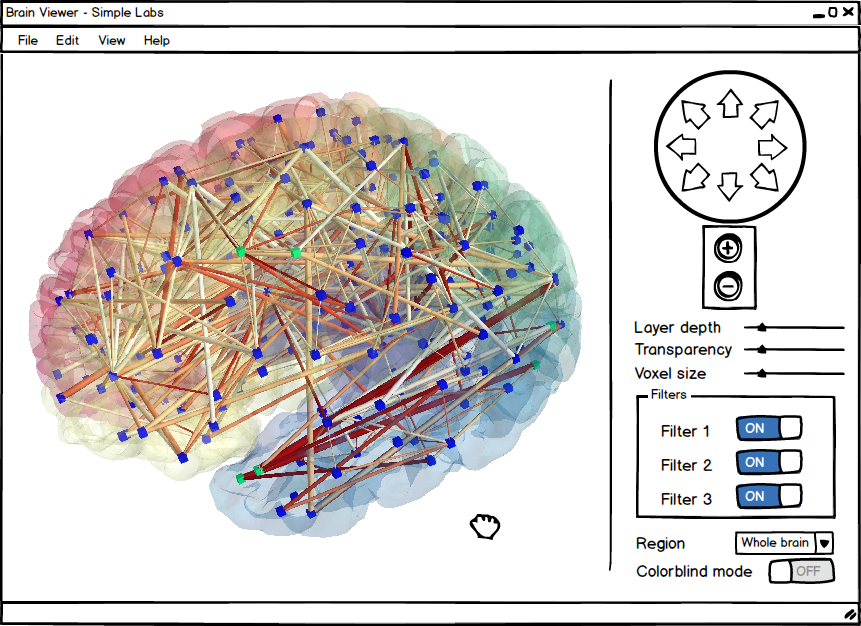
\includegraphics[width=16cm,height=9.5cm]{images/mockup1.png}
\caption{Main window}
\label{fig:mainWindow}
\end{figure}


\begin{figure}[h!]
\centering
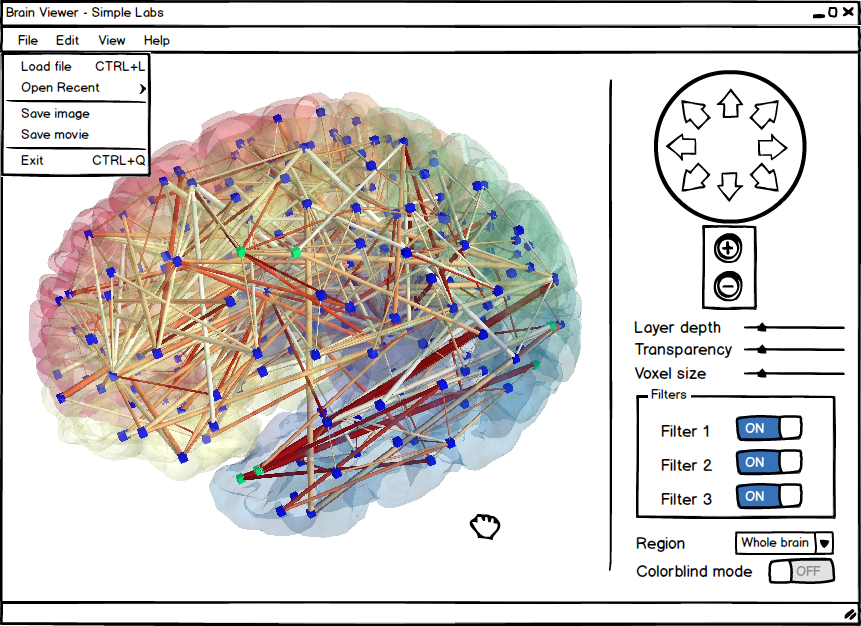
\includegraphics[width=16cm,height=9.5cm]{images/mockup2.png}
\caption{File menu}
\label{fig:fileMenu}
\end{figure}


\begin{figure}[h!]
\centering
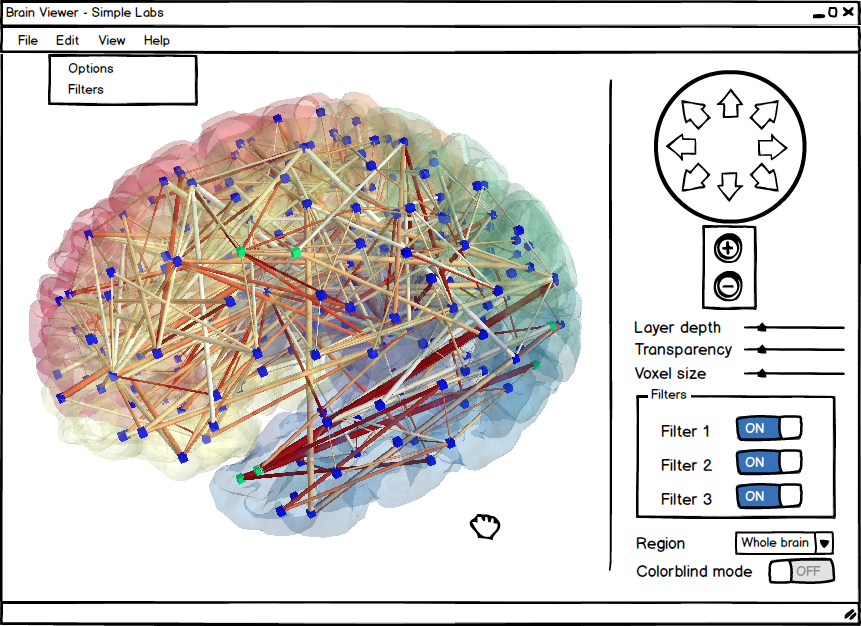
\includegraphics[width=16cm,height=9.5cm]{images/mockup3.png}
\caption{Edit menu}
\label{fig:editMenu}
\end{figure}


\begin{figure}[h!]
\centering
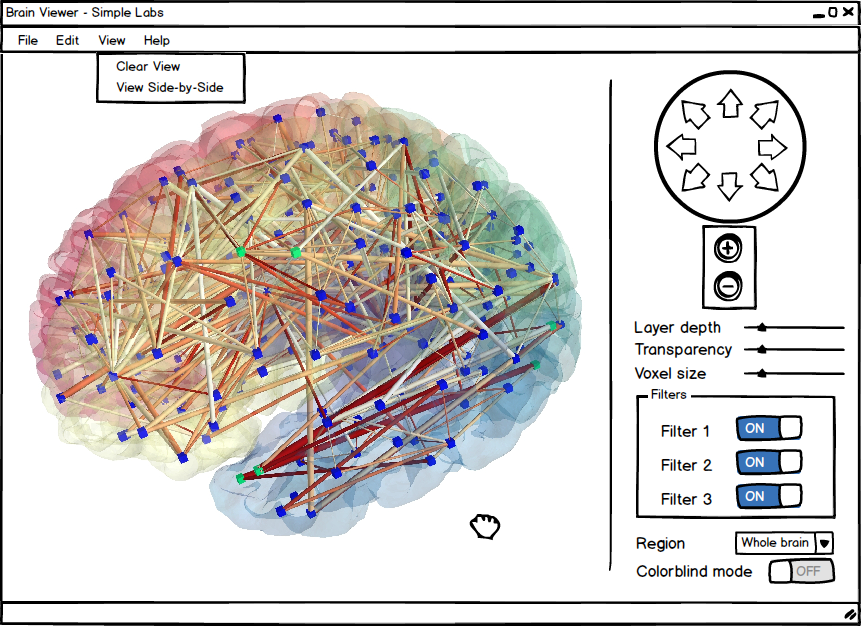
\includegraphics[width=16cm,height=9.5cm]{images/mockup4.png}
\caption{View menu}
\label{fig:viewMenu}
\end{figure}



\begin{figure}[h!]
\centering
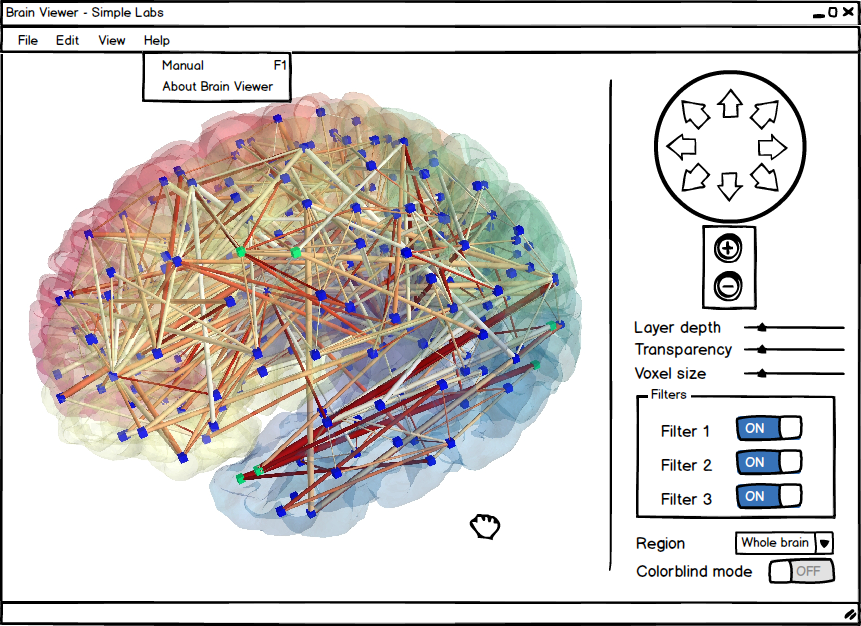
\includegraphics[width=16cm,height=9.5cm]{images/mockup5.png}
\caption{Help menu}
\label{fig:helpMenu}
\end{figure}

\newpage
\newpage
\newpage
